% !TEX root = ../thesis_main.tex

% fig:themot
% 	fig:mot
% 	fig:acmot

\begin{figure}[ht]
	\centering
	\begin{subfigure}[t]{0.242\textwidth}
		\centering
		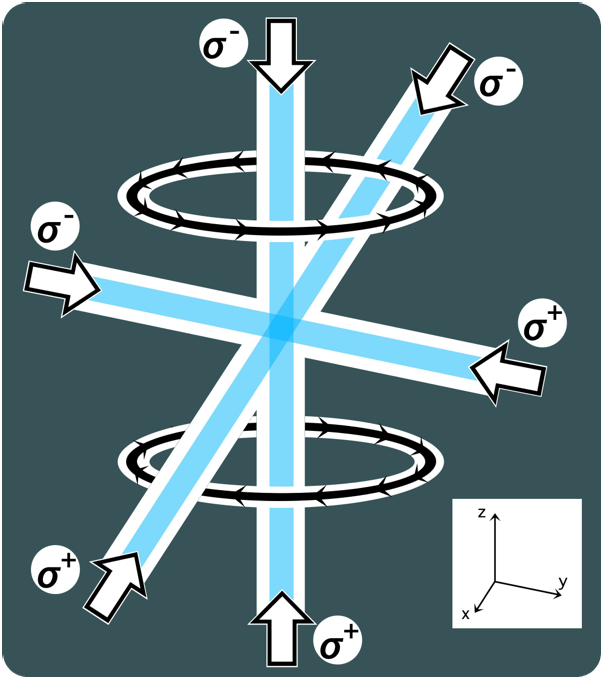
\includegraphics[width=\textwidth]{mot.png}
		\caption{Components of a magneto-optical trap, including current-carrying magnetic field coils and counterpropagating circularly polarized laser beams.}
		\label{fig:mot}
	\end{subfigure}
	\hfill
	\begin{subfigure}[t]{0.728\textwidth}
		\centering
		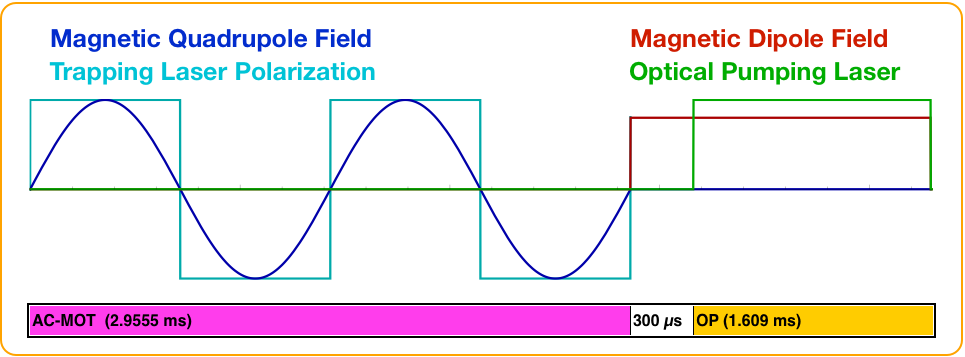
\includegraphics[width=\textwidth]{acmot.png}
		\caption{One cycle of trapping with the AC-MOT, followed by optical pumping to spin-polarize the atoms.  After atoms are transferred into the science chamber, this cycle is repeated 500 times before the next transfer.  The magnetic dipole field is created by running parallel (rather than anti-parallel as is needed for the MOT) currents through the two coils.}
		\label{fig:acmot}
	\end{subfigure}
	\caption{An alternating-current magneto-optical trap with a duty cycle optimized for producing polarized atoms}	
	\label{fig:themot}
\end{figure}
